%\begin{savequote}[8cm]
%\textlatin{Jedem Anfang wohnt ein Zauber innne.}
%
%In the core of every beginning lives magic.
%  \qauthor{--- Hermann Hesse's \textit{Stufen}}
%\end{savequote}

\chapter{\label{ch:4-DCN-LAs}Architecture Learning for Deep Counterfactual Networks} 

%\minitoc

\section{Motivation}

In the previous chapter we proposed \emph{deep counterfactual network} for the task out counterfactual inference, treating the problem as a multi-task learning problem. The network has a set of layers that are shared among both the treated and untreated outcomes and a number of outcome-specific layers. 

Nevertheless, the questions of how to select an appropriate architecture (i.e. the number of shared layers, and the number of outcome-specific layers) is of great importance and remains an open challenge. For instance, a highly unbalanced dataset with significantly different response surfaces might require an architecture that utilises a higher number of outcome-specific layers as opposed to a dataset with similar response surfaces that might perform best in an architecture with a high number of shared layers since the outcome surfaces have more commonalities. 
% TODO Should I include this as well? 
% Lastly, it is imaginable that an asymmetric architecture with different numbers for each outcome specific layer are most appropriate. 

Classical approaches involve hyper-parameter search algorithms (such as \emph{grid search}, \emph{random search}, and \emph{bayesian inference}) that can be computationally expensive. Moreover, while there are a number of optimised approaches for model selection and architecture learning in neural networks, they do not make use of the specific nature of causal inference.

% GRAPH Redo this one with big questions marks next to the hyper paramets. 
\begin{figure}[h]
	\centering
	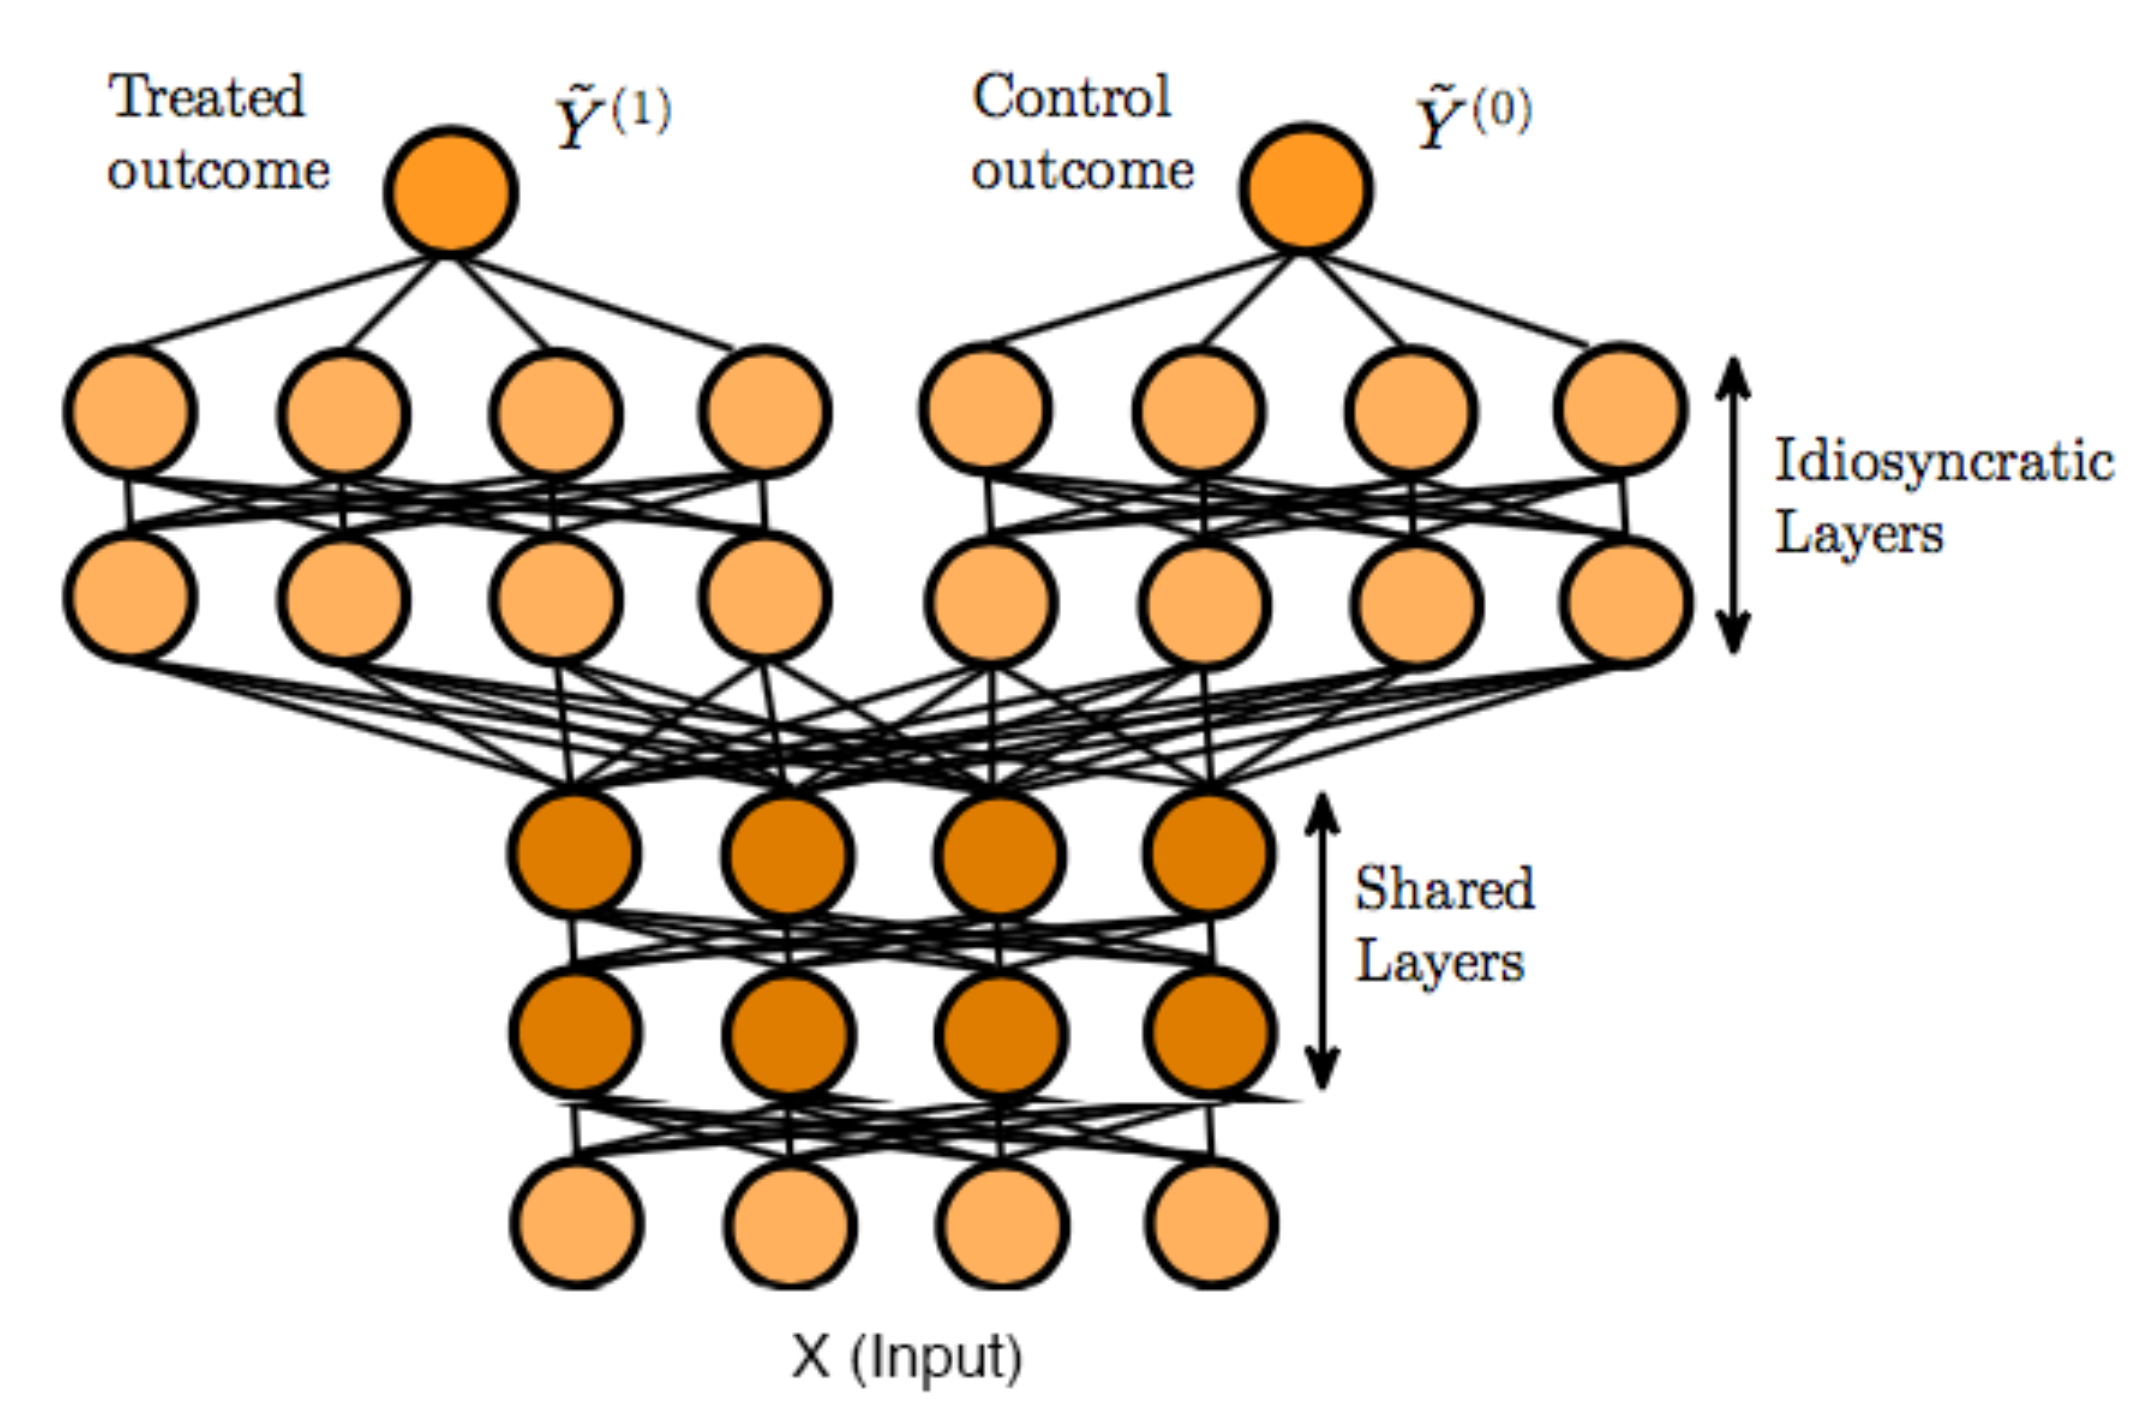
\includegraphics[width=0.8\textwidth]{figures/chapter-4/architecture-learning-motivation.png}
	\caption{Architecture Learning}\label{fig:architecture-learning-motivation}
\end{figure}

In this chapter we propose an efficient approach for automatically learning appropriate architectures of deep neural networks for the task of counterfactual inference over observational data by exploiting inferred characteristics of the dataset. For instance, if one of the outcomes in the data follows a more complex function than the other, this should be reflected in a potentially asymmetric architecture which utilises a higher number of outcome-specific layers for the this outcome.


%The approach does not rely on expensive hyper-parameter search and is achieved by exploiting inferred characteristics of the dataset such as the propensity score, the similarity between the different outcome surfaces and the individual outcome-based complexity. 


\section{Architecture Learning}
Our model is able to automatically learn a suitable architecture for the DCN by exploiting relevant characteristics of the dataset which are specific to the problem of causal inference. These characteristics such as the propensity score, the shared complexity of the response surfaces, and the individual complexity of each outcome function, can be inferred from the data to inspire a suitable architecture. This way, we achieve an efficient method of model-selection while avoiding computationally expensive hyper-parameter searches over the space of possible architectures. 

The approach is based on the observation that certain architectures are more suitable than others for the task of counterfactual inference. In particular, it can be shown empirically using traditional hyper-parameter optimisation that the best-performing architectures consistently follow specific empiric ratios between the number of shared and total layers, and the respective outcome-specific and total layers. The optimal ratios are not static, however, but depend on specific characteristics of the dataset. Once these characteristics are known, we can infer the desired number of layers and obtain a suitable architecture without the need to perform a hyper-parameter search.

In the following, we will discuss each characteristic in detail, including its intuition and formalisation. We describe how the characteristic can be inferred from the data and how it can be used to inform the architecture of the DCN.


\subsection{Relevant Characteristics} \label{sec:relevant-characteristics}
For the problem of counterfactual inference, we have identified the following main characteristics of the data. 

\subsubsection{(a) Selection Bias}
Each dataset can be considered a partition  of subjects into treated and untreated (control) subjects depending on their treatment assignment indicator $W_i$ as described in the previous section. Governed by the underlying treatment policy the dataset might be heavily imbalanced and skewed towards a specific treatment. 
Intuitively, this potential imbalance is relevant for our model because we might profit from a corresponding asymmetric architecture, i.e. a model where the number of outcome-specific layers differ from each other. 

Formally, the selection bias $\mathbf{B}$ can be quantified in terms of the average propensity score 
$$
\mathbf{B} = \frac{1}{n} \cdot \sum \limits_{{i=0}}^{n-1}  \mathbb{P}(W_i = 1 \mid X_i).
$$

The individual propensity scores can be estimated from the dataset using a neural network for which we treat the prediction of the treatment assignment as a binary classification problem in supervised learning. 



\subsubsection{(b) Similarity of  Outcome Response Surfaces}
The different outcome functions of the treated and untreated subjects can be conceptualised in terms of a shared part governed by features and their correlations that are mostly the same for both outcomes and an outcome-specific part that is inherently different. 

Intuitively, if the outcome functions are potentially complex but rather similar to each other, this should be reflected in a high number of shared layers in the network in contrast to a relatively low number of outcome-specific layers. 

Formally, we can model the different outcomes as functions
\begin{align}
\label{eqn:outcome-functions}
\begin{split}
f_1(X_i) =  \underbrace{g(X_i, \lambda^{(1)})}_{\text{shared}} +   \beta_1 \cdot \underbrace{ exp(h_1(X_i, \mu^{(1)}))}_{\text{outcome-specific}}
\\
f_0(X_i) = \overbrace{g(X_i, \lambda^{(0)})} +  \beta_0 \cdot \underbrace{exp(h_0(X_i, \mu^{(0)}))}_{\text{outcome-specific}}
\end{split}
\end{align}


where $g$ represents a common function and $h_0, h_1$ are outcome-specific (e.g. polynomial functions of different degrees). The relative weight of the shared part in comparison to the outcome-specific part is captured by $\beta_0, \beta_1 \in \mathbb{R}$ (see below). In this model, the vectors $\lambda^{(1)}, \mu^{(1)}$ represent the coefficients of a specific response surface for the factual outcome whereas we model their counterfactual counterparts as
\begin{equation}
\label{eqn:mu_and_sigma}
\lambda^{(0)}_i \sim \mathcal{N}(\lambda^{(1)}_i, \sigma)  \hspace{1cm} \mu^{(0)}_i \sim \mathcal{N}(\mu^{(1)}_i, \sigma).
\end{equation}


This way, we can use the parameter $\sigma \in \mathbb{R}_{\geq0}$ to introduce a measure of similarity $\mathbf{S} \propto \sigma$ between the two outcome surfaces. A low sigma corresponds to a high similarity which should be reflected in a large amount of shared layers, whereas an increasing sigma should result in a smaller proportion of shared layers. 

There are multiple ways to estimate $\mathbf{S}$ for a new dataset. In our approach, we train two separate feed-forward neural networks -- one exclusively for the treated subjects and one exclusively for the untreated subjects. After training, we compare the coefficients according to equation ($\ref{eqn:mu_and_sigma}$) to get an empirical estimate for $\mathbf{S}$. 
% CRITICAL This is not clear at all. How exactly do we 'compare' the coefficients? 
%TODO More precisely. What is the architecture of the networks? How do they relate to the metric above? How do we compare the coefficients. 

\subsubsection{(c) Individual Complexity of each Response Surface}
In addition to the complexity that is shared across both response surfaces, the outcomes typically possess an individual outcome-specific part that follows a completely different type of function. For instance, one of the outcomes might be linear whereas the other outcome might be a polynomial function of a higher degree. 
Intuitively, the outcome with the more complex function should have a higher number of outcome-specific layers in our model in order to capture the more complex correlations between the features, leading to an overall asymmetric architecture. 

In order to formalise the outcome-specific complexity, we use the same model for the outcome functions as defined in equations (\ref{eqn:outcome-functions}). This time we focus on the parameters $\beta_0, \beta_1 \in \mathbb{R}$ which can be used to model the relative weight that is put on the outcome-specific part in comparison to the shared part. A low value for $\beta_0$ or $\beta_1$ corresponds to a simpler individual response surface whereas higher values lead to more complex functions.  This way, we achieve a measurement of the individual outcome-complexities $\mathbf{C_0} \propto \beta_0$ and $\mathbf{C_1} \propto \beta_1$.
% CRITICAL How do I learn this? 

\subsection{Empirical Model} \label{sec:empirical-model}
Our approach is based on the observation that -- depending on the characteristics defined above -- the best-performing architectures consistently express certain empirical ratios for the different numbers of layers. This way, we can create a model $\mathcal{F}$ with 

\begin{equation}
\mathcal{F}(\mathbf{B}, \mathbf{S}, \mathbf{C_0}, \mathbf{C_1}) = \tilde{\mathbf{R}} = \begin{bmatrix}
\tilde{R_{s}} \\
\tilde{R_{i,0}} \\
\tilde{R_{i,1}}
\end{bmatrix} 
\end{equation}

that takes as input the different characteristics and outputs a vector $\tilde{\mathbf{R}}$ that contains the estimated appropriate ratios 

\begin{align} 
\tilde{R_{s}} = \frac{L_{s}}{L_{\text{total}}} && \tilde{R_{i,0}} = \frac{R_{i,0}}{L_{\text{total}}} && \tilde{R_{i,1}} =\frac{R_{i,1}}{L_{\text{total}}}
\end{align} 
between the respective layers and the total number of layers $L_{\text{total}}$. 

We train the model using  synthetically-generated datasets (see section ??) % TODO Add reference to data generation
for which we have full control over the different characteristics and use hyper-parameter optimisation such as grid-search over the set of different distributions of a fixed amount of layers to find the best-performing ratios which we then use as our target label. 


\subsection{Architecture Learning Algorithm}
Having defined and formalised the relevant characteristics of the dataset, we can derive a suitable DCN architecture for a new dataset as described in algorithm \ref{fig:algorithm}. 

First, we estimate the characteristics $\mathbf{B}$, $\mathbf{S}$, $\mathbf{C_0}, \mathbf{C_1}$ of the dataset, as described in section  \ref{sec:relevant-characteristics} (i.e. by training separate neural networks to estimate the average propensity score and the respective properties (similarity and individual complexity) of the two response surfaces). 

The estimated characteristics $\tilde{\mathbf{B}}$, $\tilde{\mathbf{S}}$, $\tilde{\mathbf{C_0}}, \tilde{\mathbf{C_1}}$ are then used as input features for our empirical model (see previous section) that was derived a priori from a hyper-parameter optimisation over a synthetic dataset. Since we cannot be sure that we receive $\tilde{R_{s}} + \tilde{R_{i,0}} + \tilde{R_{i,1}} = 1 $, we are running a \emph{softmax function} $\sigma$ which is defined as  

\begin{equation}
\sigma(\mathbf{x})_i = \frac{e^{\mathbf{x}_i}}{\sum_{k=1}^{K}e^{\mathbf{x}_k}}
\end{equation}

where $\mathbf{x}$ is a $K$-dimensional vector and $i = 1, 2, \dots, K$ on the output vector $\tilde{\mathbf{R}}$ to normalise the estimated ratios making sure they add up to $1$. 

%TODO SHould I mention that we need to multiply them now with the desired number of layers to get 


Using our approach, we can profit from the empirically suitable ratios and are able to directly estimate an appropriate architecture for our dataset $\mathcal{D}$ without the need for hyper-parameter optimisation.  

%We will refer to the \emph{deep counterfactual network} whose architecture we learned using our approach as \emph{DCN-LA}. It is trained  analogously to a traditional DCN as described in section \ref{sec:dcn-training}. 


% GRAPH Update the algorithm accordingly to reflect empirial model and vector R
\begin{algorithm}
	\caption{Architecture Learning}\label{fig:algorithm}
	\begin{algorithmic}[1]
		
		\Procedure{Architecture Learning for DCN}{} \\
		\textbf{Input:} Dataset $\mathcal{D}$, $L_{\text{total}}$  
		\State \emph{\# Learn Characteristics from dataset}
		\State $\ \tilde{\mathbf{B}} \gets \textit{estimate selection bias (a)}$
		\State $\ \tilde{\mathbf{S}} \gets \textit{estimate response surface similarity (b)}$
		\State $\ \tilde{\mathbf{C_0}}, \tilde{\mathbf{C_1}} \gets \textit{estimate individual complexity (c)}$\\
		\State \emph{\# Derive Architecture}
		\State $\ {L_s} \gets \tilde{L_s}(\tilde{\mathbf{B}}, \tilde{\mathbf{S}}, \tilde{\mathbf{C_0}}, L_{\text{total}})$
		\State $\ {L_{i,0}}\gets \tilde{L_{i,0}}(\tilde{\mathbf{B}}, \tilde{\mathbf{S}}, \tilde{\mathbf{C_0}}, L_{\text{total}})$
		\State $\ {L_{i,1}}\gets \tilde{L_{i,1}}(\tilde{\mathbf{B}}, \tilde{\mathbf{S}}, \tilde{\mathbf{C_1}}, L_{\text{total}})$ \\
		\textbf{Return:} $L_s, L_{i,0}, L_{i,1}$ 
		
		\EndProcedure
	\end{algorithmic}
\end{algorithm}

	